\subsection{Differential Chromatic Refraction}
\label{sec:diffeerential_chromatic_refraction}

Differential chromatic refraction (DCR) occurs when light passes through Earth’s atmosphere, refracting more for shorter wavelengths, which causes blue light to appear shifted closer to the zenith. This wavelength-dependent effect results in the smearing of point sources along the zenith direction, specifically parallel to the parallactic angle. The DCR effect is observable in LSST ComCam data, particularly in the angular offset versus g-i band magnitude difference plots (Figure \figRef{dcr}). Figure \figRef{dcr} contains all direct sources with SNR > 10 from 41 visits from November 26, 2024. When looking at data perpendicular to the parallactic angle, sources show no DCR effect (as expected), forming a clear vertical distribution on the hexbin plots. In contrast, sources parallel to the parallactic angle exhibit a tilted, linear distribution, clearly demonstrating the relationship between angular offset and the g-i band magnitude difference—a visual indication of the DCR effect.

\begin{figure}
  \centering
  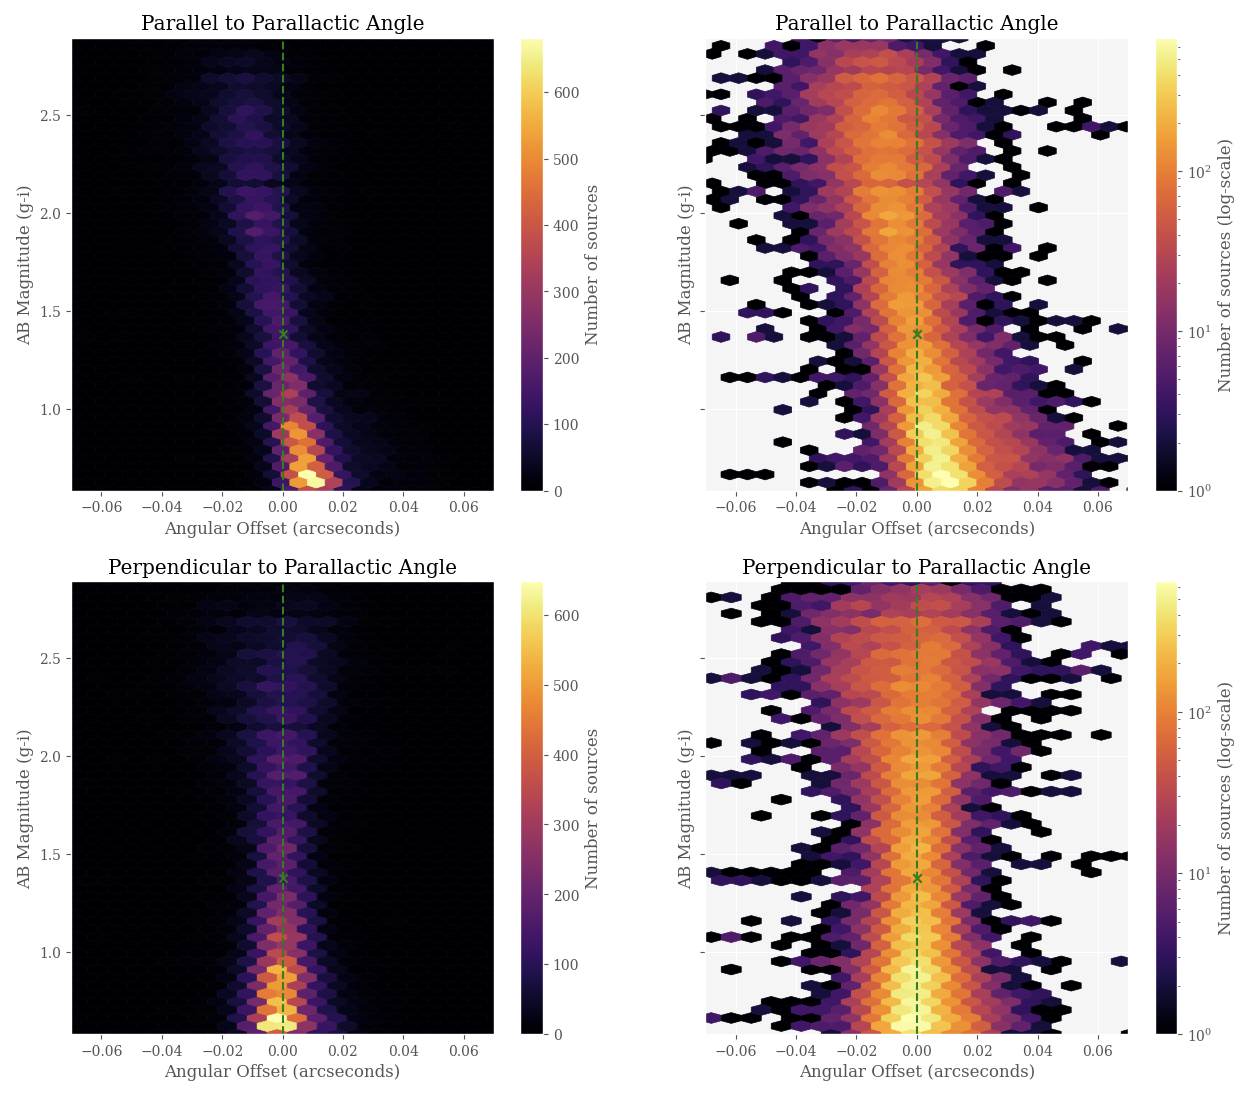
\includegraphics{dcr_figures/dcr_plot1.png}
  \caption{Visualization of Differential Chromatic Refraction (DCR) observed in the ComCam commissioning campaign. The g-i color is computed for every source in the reference catalog that is matched to a direct source in the science image, and the binned density for the full survey is plotted against the angular offset between the reference and detected positions. The angular offset is projected along coordinates parallel and perpendicular to the parallactic angle of the observation, and shows a characteristic correlation along the parallel axis with no correlation along the perpendicular axis. The green vertical dashed line indicates the expected g-i magnitude distribution at zero angular offset, while the green ‘x’ marks the average g-i magnitude of the plotted sources.}
  \label{fig:dcr}
\end{figure}

